\section{Introduction}
\label{section:hardware: introduction}

%\textbf{Benjamin: I think, a more general introduction is needed before one dives into the radiometer equation.}

\subsection{Basics of RFI in radio astronomy}
The radiometer equation is fundamental in radio astronomy for determining the sensitivity of a radio telescope. It quantifies the sensitivity of a radio telescope as a function of the receiver system temperature, bandwidth, and observation time, offering insight into the minimum detectable signal. The equation is given by:
\[ \Delta S = \frac{2 k_B T_{\text{sys}}}{A_{\text{eff}} \sqrt{2 \Delta f \tau}} \]
where \( \Delta S \) is the minimum detectable flux density in Jansky (1 Jy = $10^{-26}$Wm$^2$Hz$^{-1}$), \( k_B =1.38 \times 10^{-23} \;\text{J} / \text{K}\) is the Boltzmann constant, \( T_{\text{sys}} \) is the system temperature in Kelvin (K), \( A_{\text{eff}} \) is the effective area of the telescope in $m^2$, \( \Delta f \) is the observed bandwidth in Hz, and \( \tau \) is the integration time in seconds (s). This equation highlights the importance of maintaining a low system temperature, utilising a large effective area, operating over a broad bandwidth, and employing a long integration time to enhance the sensitivity and accuracy of astronomical observations.

In the context of interferometry, where signals are correlated between pairs of antennas rather than detected by a single dish, the sensitivity of a single visibility measurement is given by the interferometric radiometer equation:

\[ \Delta S = \frac{2 k_B T_{\text{sys}}}{\eta_s A_{\text{eff}} \sqrt{ \Delta f \, \tau }} \]

Here, $\eta_s$ is the system efficiency factor, typically close to unity. The absence of the $\sqrt{2}$ factor (compared to the single-dish case) reflects that real and imaginary components of visibilities are treated separately. In an array with $N$ antennas, the overall image sensitivity improves with the number of independent baselines, scaling approximately as $\sqrt{N(N-1)}$ for a complete array.

These two forms of the radiometer equation form the theoretical foundation for quantifying sensitivity and for designing optimal observational strategies in radio astronomy. The sensitivity that modern radio astronomy systems can achieve is unrivalled in other radio services and applications. However, this fantastic achievement also comes at a cost. Observations are highly susceptible to various human-made transmissions and other forms of electromagnetic radiation. A cell phone on the Moon would be among the brightest sources in the sky, at the respective frequencies. 

The sensitivity requirements of modern radio astronomy compel astronomers to explore frequencies well beyond the protected passive bands owing to the scarcity, limited bandwidth, and incomplete coverage of these designated ranges. Astronomers usually refer to the anthropogenic signals found beyond these protected bands as RFI. Still, it has to be pointed out that in legal terms, most of the disturbing features in the radio telescope data are not considered as RFI by administrations and other spectrum management stakeholders, as the operators of radio transmitters usually have a license, and the wanted transmissions, e.g., cell phone carriers, are perfectly legal. In spectrum management, RFI specifically means any kind of unwanted emission, such as near-spectral sidelobes, harmonics or intermodulation products, which can leak into the allocated band of another radio service.

While the Radiocommunication Sector of the International Telecommunication Union (ITU-R) has acknowledged the requirements of radio astronomy decades ago, the total amount of spectrum that is allocated to the Radio Astronomy Service (RAS) is low. As a consequence, in addition to measurements in the RAS bands, we are opportunistic -- observing the parts of the spectrum outside of the protected bands wherever and whenever possible at an observatory, as not every active radio service is equally utilised everywhere. 

With more and more digital transmissions, however, the efficiency of spectrum usage has increased significantly in recent years. Therefore, the need increases to deal with human-made features in our datasets, which can range from flagging affected data samples to attempting to fully remove them.

Generally, in radio astronomy, RFI is classified based on spectral occupancy. The primary classification is broadband and narrowband. An example of broadband and narrowband RFI is shown in Figure~\ref{fig:ugmrt-rfi}.

It should be noted that the best form of interference mitigation is still to avoid them in the first place. Radio astronomers have done their part by constructing telescopes in the most remote locations physically accessible, with as little radio noise background as possible. Often, site searches entailed dedicated spectrum monitoring to find the quietest places. Making use of terrain shielding provides additional protection. Furthermore, astronomers participate in national and international spectrum management forums such as the International Telecommunication Union (ITU) to advocate for protection from new applications in the bands allocated to the RAS.

Only if all these efforts fail -- and this is mostly the case -- actual RFI mitigation needs to be considered.

%An example of narrowband and broadband RFI as seen in the spectrogram of uGMRT is shown in Figure.

\begin{figure}
    \centering
    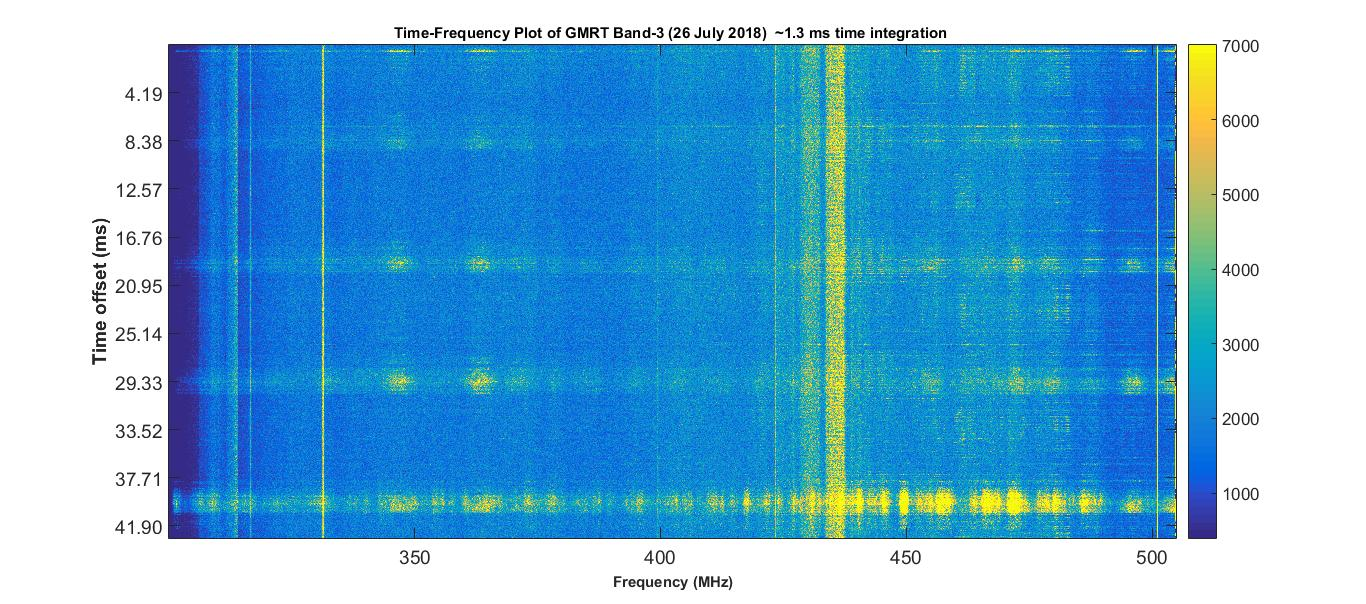
\includegraphics[scale=0.25]{Hardware Excision Techniques/figures/time_freq(1).jpg}
    \caption{Spectrogram of upgraded Giant Metrewave Radio Telescope (uGMRT) \citep{gupta2017upgraded} antenna showing broadband (powerline RFI) and narrowband (communication transmitters) RFI in the 250-500 MHz band. Broadband powerline RFI is seen to be repeated every 10ms (submultiple of 50Hz powerline frequency). Note that the astronomical signal is buried below the noise floor and cannot be identified in this plot.}
    \label{fig:ugmrt-rfi}
\end{figure}




\subsection{Levels of RFI}
\label{subsection:hardware:introduction: levels}
A radio astronomy receiver chain begins with a feed that collects celestial radio waves, directing them to a low-noise amplifier (LNA). The LNA amplifies these weak signals with minimal added noise, ensuring data integrity. After amplification, the signal passes through a bandpass filter to isolate the frequency of interest, followed by downconversion, when applicable, to an intermediate frequency (IF) using a mixer and local oscillator. The IF or baseband signal is further amplified, filtered, and digitized by an analog-to-digital converter (ADC), though modern systems increasingly digitize directly at the radio frequency (RF) to minimize signal degradation.

RFI impacts the receiver chain at varying levels:
\begin{itemize}
%\item \emph{Level 0}: Undetectable RFI does not impact observations, requiring long integration times to assess its threshold via modelling or experiments.
\item \emph{Level 0}: RFI that appears undetectable relative to the system sensitivity. While such signals may fall below the detection threshold in a single observation, they can still introduce subtle biases, particularly in statistical or detection-limited experiments near the noise floor, through persistent systematic effects. According to the radio interferometer measurement equation, even low-level signals can bias results if they correlate with the observing process. Thus, \emph{Level 0} should be understood as RFI whose power spectral density is at least an order of magnitude below the sensitivity threshold of the instrument. It is often referred to as “unaffecting RFI,” though its actual impact may only be assessable through long integrations or modelling.
\item \emph{Level 1}: Detectable RFI adds unwanted contributions, requiring excision to preserve data integrity, but this can reduce sensitivity and hinder the detection of sparse astronomical signals or calibration accuracy.
\item \emph{Level 2}: Stronger RFI pushes the LNA into non-linear operation, generating harmonics and intermodulation products. Mitigation involves excising data and using attenuators, further degrading sensitivity.
\item \emph{Level 3}: Severe RFI causes ADC saturation, resulting in irrecoverable signal artefacts. Mitigation typically includes attenuators at the cost of a loss in sensitivity or ADC direct sampling with a high dynamic range.
\item \emph{Level 4}: Extreme RFI physically damages receiver components, requiring the telescope to cease operation.
\end{itemize}
%Spectrum management aims to ensure Level 0 RFI across primary radio astronomy frequency bands while recognizing that all levels of RFI may occur in non-allocated bands, depending on the telescope's environment. This balance reflects the ongoing challenges in protecting sensitive radio astronomy observations from both in-band and out-of-band emissions.
Spectrum management aims to ensure RFI remains at or below Level 0 within primary radio astronomy bands as defined by international allocations, as well as within nationally or voluntarily protected zones such as Radio Quiet Zones (RQZs). In these cases, signals may fall below the threshold to be considered interference at all. Outside of these protected bands or regions, all levels of RFI may occur depending on the local spectral environment. This highlights the persistent challenge of protecting sensitive radio astronomy observations from both in-band and out-of-band emissions.



\subsection{Motivation for real-time RFI mitigation}
\label{subsection:hardware:introduction: motivations}

RFI mitigation in a radio observatory is carried out in different ways \citep{ford2014rfi}. Real-time RFI mitigation usually happens in the analog domain or at the highest time resolution, i.e. close to the Nyquist rate, which helps minimize the data corruption due to sparse RFI in downstream signal processing with minimal loss of astronomical data, thereby improving and enhancing the quality and accuracy of astronomical measurements. Other benefits from real-time RFI mitigation are as follows:

\begin{enumerate}
\item For time-domain impulsive RFI, the energy spreads across the observing band in the frequency domain, making it impossible to mitigate in the spectral or post-correlation domain.  See Figure~\ref{fig:rfi_example_radar} for an illustration of a radar system.

\item Correlated RFI is best treated in the pre-correlation domain to reduce its ill effects on the astronomical data.

\item RFI is mostly non-random; hence, its early removal helps follow the radiometer equation, which is crucial to achieving the desired sensitivity of the telescope.

\item It helps facilitate adjustments to the telescope signal processing chain in response to a dynamic RFI environment. This adaptability is crucial in maintaining the continuity of observations and ensuring that data collection is optimized even in transient or sporadic RFI.
\end{enumerate}

%\subsection{RFI classification}
%\label{subsection:hardware:introduction: classification}
Figure~\ref{fig:real-time-rfi} illustrates the increase in data loss in a typical radio telescope receiver signal processing chain.

\begin{figure}
    \centering
    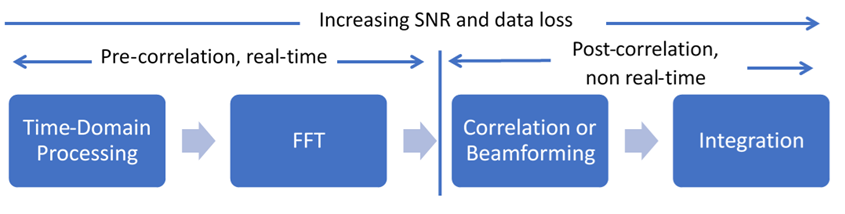
\includegraphics[scale=0.8]{Hardware Excision Techniques/figures/rt.jpg}
    \caption{SNR versus data loss in a typical telescope receiver system}
    \label{fig:real-time-rfi}
\end{figure}


\begin{figure}
    \centering
    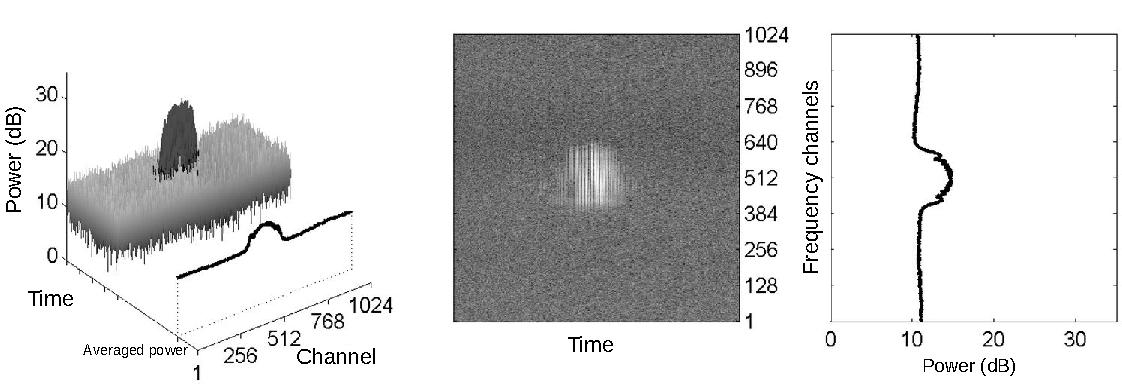
\includegraphics[height=.20\textheight]{figures/radar.pdf}
    \caption{One of the 5-s periodic bursts received from a radar system.  The burst is a group of many periodic short impulses, sparse in time, but broad.  }
    \label{fig:rfi_example_radar}
\end{figure}

Real-time RFI mitigation strategies fall into three broad categories: \textit{excision}, \textit{subtraction}, and \textit{coordination}. Excision techniques identify and remove contaminated samples before averaging, reducing downstream corruption but resulting in irreversible data loss and potential statistical biases \citep{hugo2022tricolouroptimizedsumthresholdflagger,10464448}. Subtraction methods attempt to preserve the astronomical signal by estimating and removing the interference, yet are limited by residuals due to imperfect modelling and front-end nonlinearities \citep{ellingson2022coherent,chakraborty2024low}. Coordination approaches mitigate RFI proactively—e.g., via predictive scheduling or emitter cooperation—but may constrain telescope operations \citep{hellbourg2024assessing}. These trade-offs are summarized in Table~\ref{real-time-tech}.



%Additionally, real-time RFI mitigation contributes to the protection and longevity of sensitive receiver components by promptly handling high-power interfering signals and reducing the risk of thermal damage and long-term degradation of electronic components.
%While real-time detection and excision of RFI is beneficial in radio astronomy, it comes with challenges. The main challenge is the cost and power consumption. Even though RFI has become a significant threat to radio astronomy for several decades, few signal chains of radio telescopes have been designed considering the real-time excision of RFI. Hence, the real-time RFI excision methods deployed in existing radio telescopes are implemented using the remaining resources after implementing the key signal processing modules and operated with limited power. Regarding quality, one of the main checks that needs to be made is the flagging duration and accuracy of flagging.  It should be ensured that the excision is optimal i.e. there is no over-excising of the data, which can result in the loss of precious observational data or under-excising, which leads to RFI remnants in the data.


%An example of a real-time RFI mitigation released and operational for the uGMRT, including the possibility of extending it to contemporary and upcoming telescopes, is provided in \citep{buch2023real}.


%\subsection{Advantages of Real-Time RFI Excision}
%\label{subsection:hardware:introduction:advantages}

%Advantages of Real-Time RFI Excision
%Improved Data Quality: By removing RFI in real-time, astronomers can obtain cleaner data, which can lead to more accurate and reliable scientific results.
%Reduced Storage Requirements: Removing RFI before data is stored can significantly reduce the amount of storage space required, as only the cleaned data needs to be preserved.
%Real-Time Monitoring: Real-time excission allows astronomers to monitor the data quality as it is being collected, enabling them to identify and address potential issues promptly.
%Efficient Data Analysis: Clean data is easier and more efficient to analyze, as it is less likely to be contaminated by artifacts or noise.
%Reduced Computational Burden: By removing RFI before data is analyzed, astronomers can reduce the computational resources required for subsequent processing.

%\%subsection{Challenges of Real-Time RFI Excision}
%\label{subsection:hardware:introduction:challenges}

%Disadvantages of Real-Time RFI Excision
%Algorithm Complexity: Developing accurate and efficient algorithms for real-time RFI excission can be challenging, especially for complex RFI patterns.
%Computational Overhead: Real-time excission can introduce computational overhead, which may limit the data throughput of the telescope.
%Risk of False Positives and Negatives: There is a risk of mistakenly removing genuine astronomical signals or leaving RFI in the data, which can impact the scientific interpretation.
%Dependency on Algorithm Performance: The effectiveness of real-time RFI excission depends heavily on the performance of the algorithms used, which can be affected by factors like the type and severity of RFI.
%Potential for Data Loss: In some cases, aggressive RFI excission can lead to the loss of genuine astronomical signals, particularly if the RFI is difficult to distinguish from the signal.


%\subsubsection{Thushara}
%Real-time RFI excision enables radio astronomers to salvage observations taken in a contaminated segment of the observation band, either when the RFI source is not transmitting or when the RFI strength is attenuated to a level below the ITU recommended threshold\citep{ITU_protection_2003}. For example, consider the interference caused by strong radio pulses emitted by the Distance Measuring Equipment (DME) of an aircraft \citep{wiki_dme_2024}, which are being picked up by the antennas of radio telescopes. The DME pulses transmit in bands within 960-1215 MHz at a power level of 1 kW. Each DME pulse is 3.5 µs wide and repeats every 12 µs for a second or so in a single burst. Normally, the DME pulses are detected by the sidelobes of the antennas of a radio telescope. These pulses can be fairly easy to detect at the front of the signal chain of the radio telescope, which is operating at a wider bandwidth. Once detected, the contaminated data can be flagged in real-time to prevent further contamination of the accumulation. Also, RFI detection carried out along the various stages of the signal chain of a radio telescope allows radio astronomers to maintain the linearity of the signal chain with proper scaling while achieving the maximum possible dynamic range for a given set of computational resources.

%While real-time detection and excision of RFI is beneficial in radio astronomy it comes with challenges. The main challenge is the cost and power consumption. Even though RFI has become a significant threat to radio astronomy for several decades or so few signal chains of radio telescopes have designed considering the real-time excision of RFI. Hence, the real-time RFI excision methods deployed in existing radio telescopes are implemented using the remaining resources after implementing the key signal processing modules and operated with limited power. In terms of quality, one of the main drawbacks of real-time RFI excision is the uncertainty of the flagging duration.  This leads to either over-excising the data resulting in the loss of precious observations or under-excising which leads to RFI remnants causing artifacts in the observations. 

%\subsubsection{Kaushal - Motivation for Real-time RFI Mitigation}

%Real-time RFI mitigation usually happens at the highest time resolution (Nyquist rate) which helps prevent data corruption in downstream signal processing with minimal loss of astronomical data. Other benefits from real-time RFI mitigation are as follows:

%1. For time-domain impulsive RFI, the energy 
%spreads across the observing band upon Fourier
%transformation, making it difficult to detect and
%mitigate in the post-processing operation.

%2. Mitigation in the pre-correlation domain helps
%reduce the ill effects of correlated RFI.

%3. RFI is mostly non-random and hence its early removal helps in following the radiometer equation which is crucial to achieve the desired sensitivity of the telescope.

%\subsubsection{Greg}
%Real-time RFI mitigation is a critical capability of modern radio telescopes that facilitates adjustments to the telescope signal processing chain in response to a dynamic RFI environment. This adaptability is crucial in maintaining the continuity of observations and ensuring that data collection is optimized despite the presence of transient or sporadic RFI. It also enhances the quality and accuracy of the collected astronomical information by identifying, attenuating, or excising corrupted data at the highest data rates before any data compression, and preventing the saturation of the vulnerable receiver components (e.g. LNA or ADC).

%Mitigating RFI in real-time also helps minimizing the downstream computational load and storage requirements by processing the RFI contribution at the point of data acquisition rather than further down the signal chain. This strategy alleviates the need for storing intermediate data products, which can be unbearbel with the increase of telescope bandwidths and array sizes.

%Additionally, real-time RFI mitigation contributes to the protection and longevity of sensitive receiver components by promptly handling high-power interfering signals and reducing the risk of thermal damage and long-term degradation of electronic components.

